\documentclass{book}
\usepackage[utf8]{inputenc}  
\usepackage[T1]{fontenc}  
\usepackage[francais]{babel}
\usepackage{amsmath}  
\usepackage{amssymb}
\usepackage{amsfonts}
\usepackage{graphicx}
\usepackage{float}
\usepackage{dsfont}


\usepackage{geometry}
\geometry{hmargin=2.5cm,vmargin=1.5cm}

\begin{document}

\appendix

\chapter{La formule de \textsc{Breguet}}
La formule de \textsc{Breguet} est une formule mathématique fondamentale en aérodynamique. Elle relie la consommation de fuel aux paramètres de l'avion et opérationnels de la manière suivante :
\[M_{fuel}=(M_{empty}+M_{pload})\left(e^{\frac{SFC.g.R_a}{VF}10^{-3}}-1\right)\]
où
\begin{itemize}
\item $M_{empty}=42600kg$ la masse à vide de l'avion
\item $M_{pload}=62500kg$ la masse maximale de l'avion
\item $g=9.8m.s^{-1}$ la constante gravitationnelle 
\item $R_a=3000km$ la distance parcourue
\end{itemize}
sont des constantes
et 
\begin{itemize}
\item $V$ la vitesse de croisière
\item $F$ "lift to drag ratio" (finesse)
\item $SFC$ "specific fuel consumption" 
\end{itemize}
sont des variables aléatoires.

\vspace{1\baselineskip}
Plus précisément :
\begin{itemize}
\item $V$ suit une loi uniforme sur $[226, 234]$
\item $F$ suit une loi Bétâ de paramètres (7,2) sur l'intervalle $[18.7, 19.05]$
\item $SFC$ a la densité $h(x)=3.45e^{-3.45(x-17.23)}\mathds{1}_{[17.23,+\infty[}(x)$
\end{itemize}
\vspace{1\baselineskip}

Le script R \texttt{echantillon.R} propose 4 fonctions pour simuler des $N$-échantillons des différentes variables aléatoires. Un $N$-échantillon de $M_{fuel}$ est simulé en simulant d'abord un $N$-échantillon de $F$, $V$, et $SFC$ puis en utilisant la formule de \textsc{Breguet}.

\chapter{Précision sur la loi de $F$}
L'énoncé du BE nous apprend que $F$ suit une loi Bétâ $(\alpha, \beta)$ sur un intervalle $[a, b]$.
Cependant, après avoir vérifié la vraissemblance des formules de densité proposées dans l'énoncé, la densité de $F$ comporte une erreur.
En effet, en intégrant la densité sur $\mathbb{R}$ avec la mesure de Lebesgue, on devrait obtenir 1. Or selon l'énoncé, la densité de la loi de $F$ est 
\[g(x) = \frac{(x-a)^{\alpha-1}(b-x)^{\beta-1}}{(b-a)^{\beta -1}B(\alpha,\beta)}\mathds{1}_{[a,b]}(x)\]
En intégrant sur $\mathbb{R}$:
\begin{align*}
\int_\mathbb{R} g(x) \, \mathrm{d}x &= \int_{a}^{b} \frac{(x-a)^{\alpha-1}(b-x)^{\beta-1}}{(b-a)^{\beta -1}B(\alpha,\beta)} \, \mathrm{d}x\\
\intertext{changement de variable $x=u(b-a)+a$ avec $u$ sur $[0,1]$ et $\mathrm{d}x=(b-a)\mathrm{d}u$}
        &= \int_{0}^{1}\frac{(u(b-a)+a-a)^{\alpha-1}(b-u(b-a)-a)^{\beta-1}}{(b-a)^{\beta -1}B(\alpha,\beta)}(b-a) \, \mathrm{d}u \\
        &= \frac{(b-a)^{\alpha-1}(b-a)^{\beta-1}(b-a)}{(b-a)^{\beta-1}} \underbrace{\int_0^1\frac{u^{\alpha-1}(1-u)^{\beta-1}}{B(\alpha,\beta)}\, \mathrm{d}u}_{=1} \\
        &= (b-a)^{\alpha} \\
        &\neq 1
 \end{align*}
 
On en conclut que
\[g(x) = \frac{(x-a)^{\alpha-1}(b-x)^{\beta-1}}{(b-a)^{\alpha + \beta -1}B(\alpha,\beta)}\mathds{1}_{[a,b]}(x)\]
serait une densité convenable pour $F$.

Cette erreur est présente dans l'énoncé du BE mais aussi dans le document ~\cite{ref2}.

\chapter{Description des variables}
Dans cette annexe, on voulait présenter les histogrammes des échantillons $V$, $F$ et $SFC$. Il ne semblait pas pertinent de les inclure dans le corps principal du BE car leurs propriétés sont connues (les lois étant connues) mais ils permetteraient de constater l'adéquation entre les réalisations des variables et les densités théoriques qui ont permies de les simuler. Cependant, un problème du logiciel R irrésolu malgré de longues tentatives répétées reposant sur un défaut persistant de normalisation en fréquence des histogrammes (fonction \texttt{hist}) n'a pas permis d'obtenir ces graphes. On propose alors à la place les graphes des fonctions de répartition des variables $V$, $F$ et $SFC$. Ceux-ci ne permettent peut-être pas une aussi bonne visualisation de la répartition des échantillons mais sont tout autant pertinents mathématiquement pour montrer l'adéquation (en loi) entre les échantillons empiriques et les lois théoriques.

\begin{center}
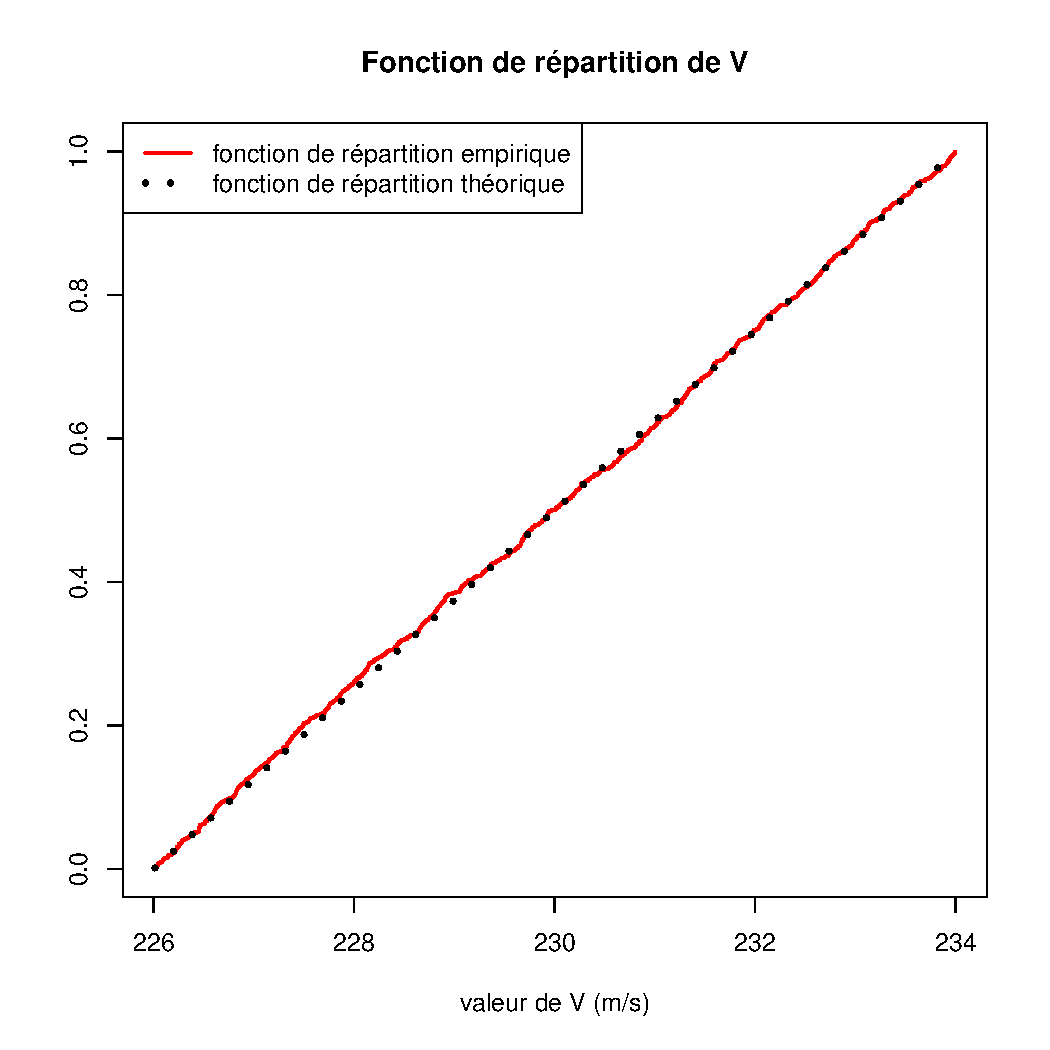
\includegraphics[scale=0.7]{V_fctrep.pdf}
\end{center}\begin{center}
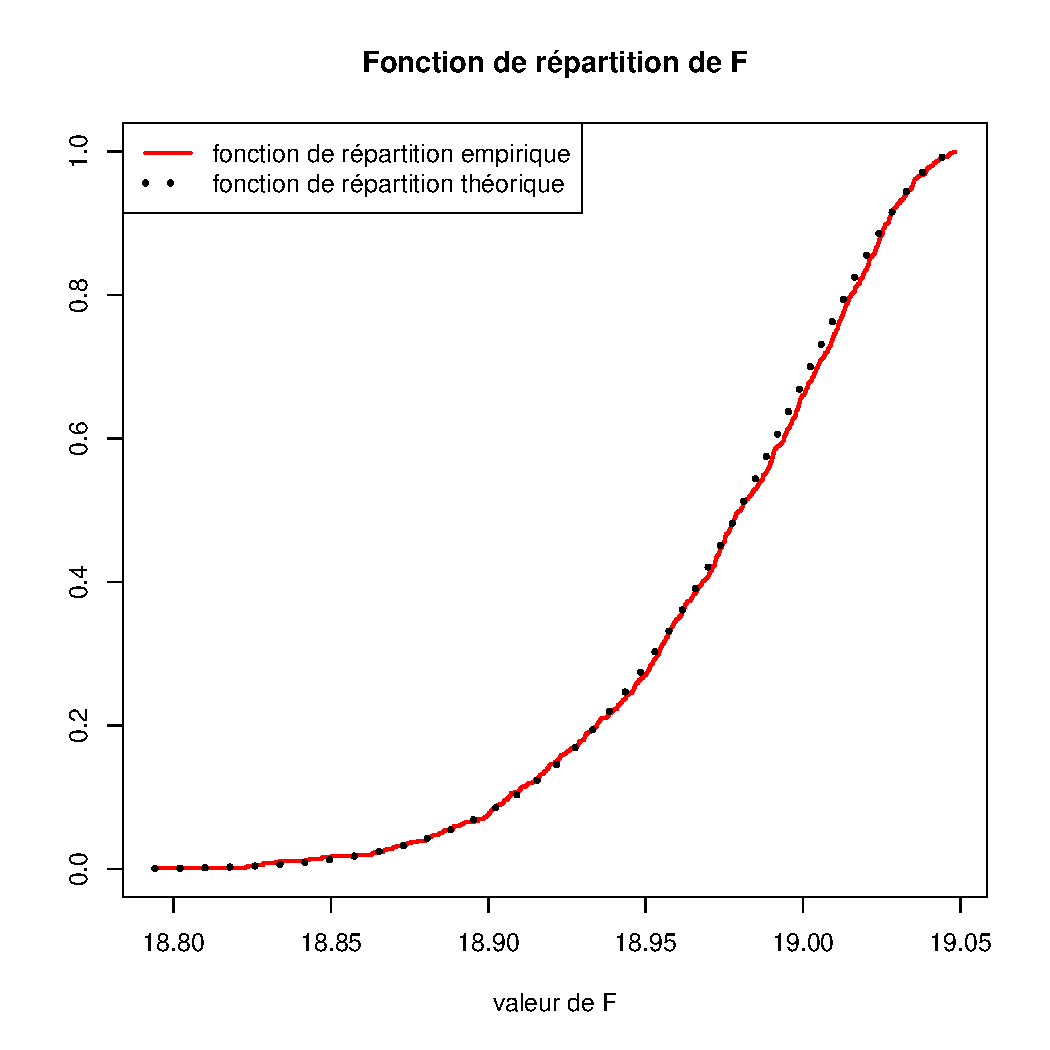
\includegraphics[scale=0.7]{F_fctrep.pdf}
\end{center}\begin{center}
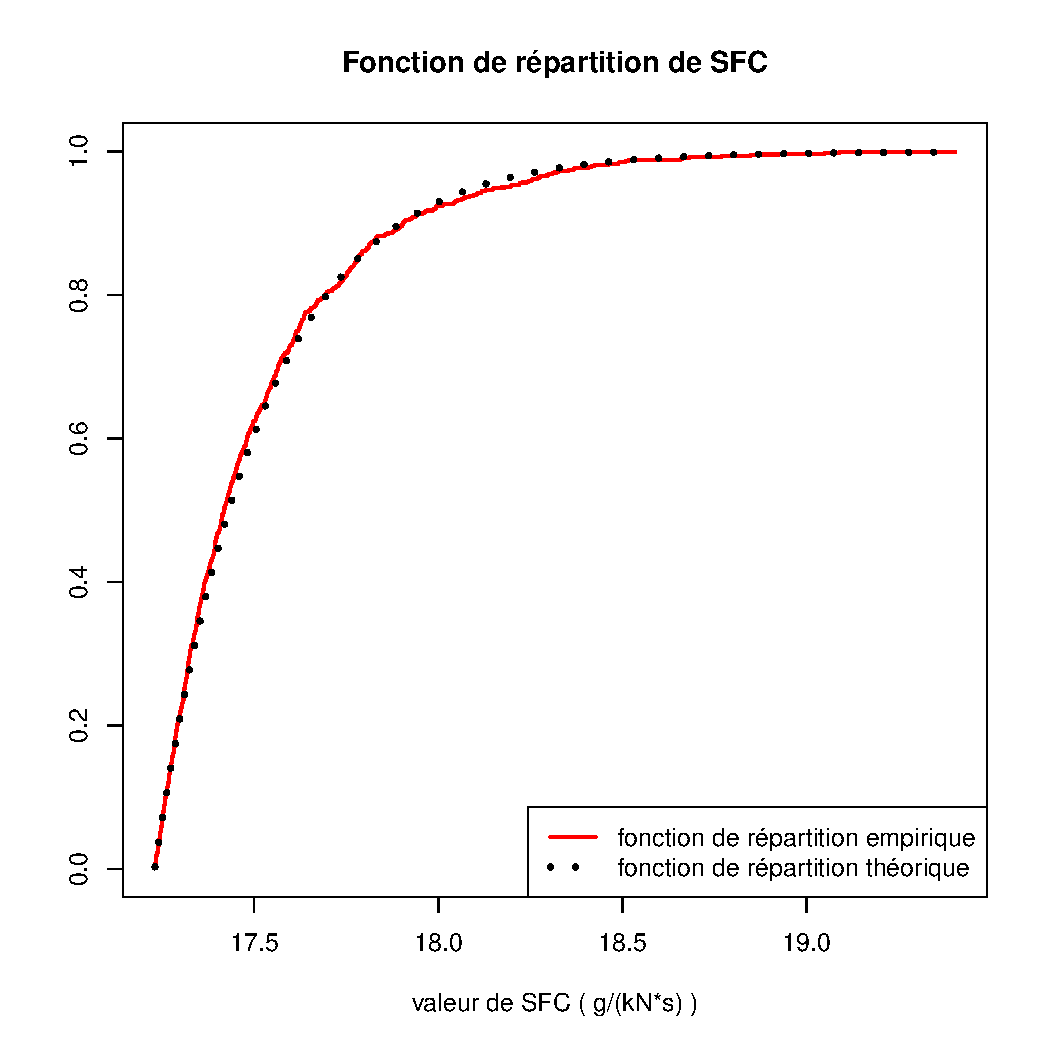
\includegraphics[scale=0.7]{SFC_fctrep.pdf}
\end{center}
Constatons la superposition entre la fonction de répartition théorique et l'empirique.

\medbreak
On présente également un diagramme boite-à-moustaches (Box-plot) d'un $N$-échantillon de $M_{fuel}$ et la fonction de répartition estimée de $M_{fuel}$ afin de mieux décrire la seule vaiable pour laquelle il n'est pas donné de modèle théorique. Ces graphes sont répétés avec des niveaux de bruit ("bruit" signifie $\sigma$) différents. 
\begin{center}
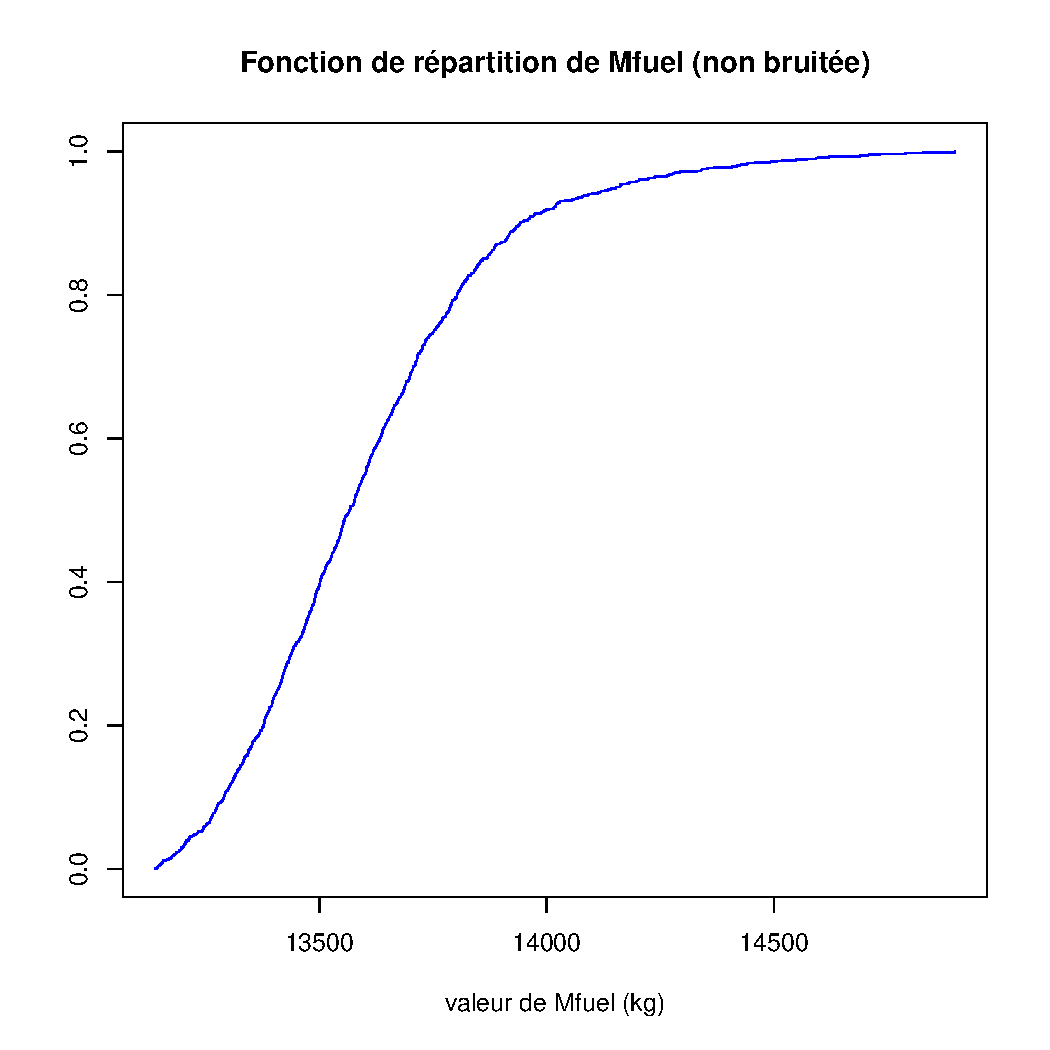
\includegraphics[scale=0.7]{M_fctrep.pdf}
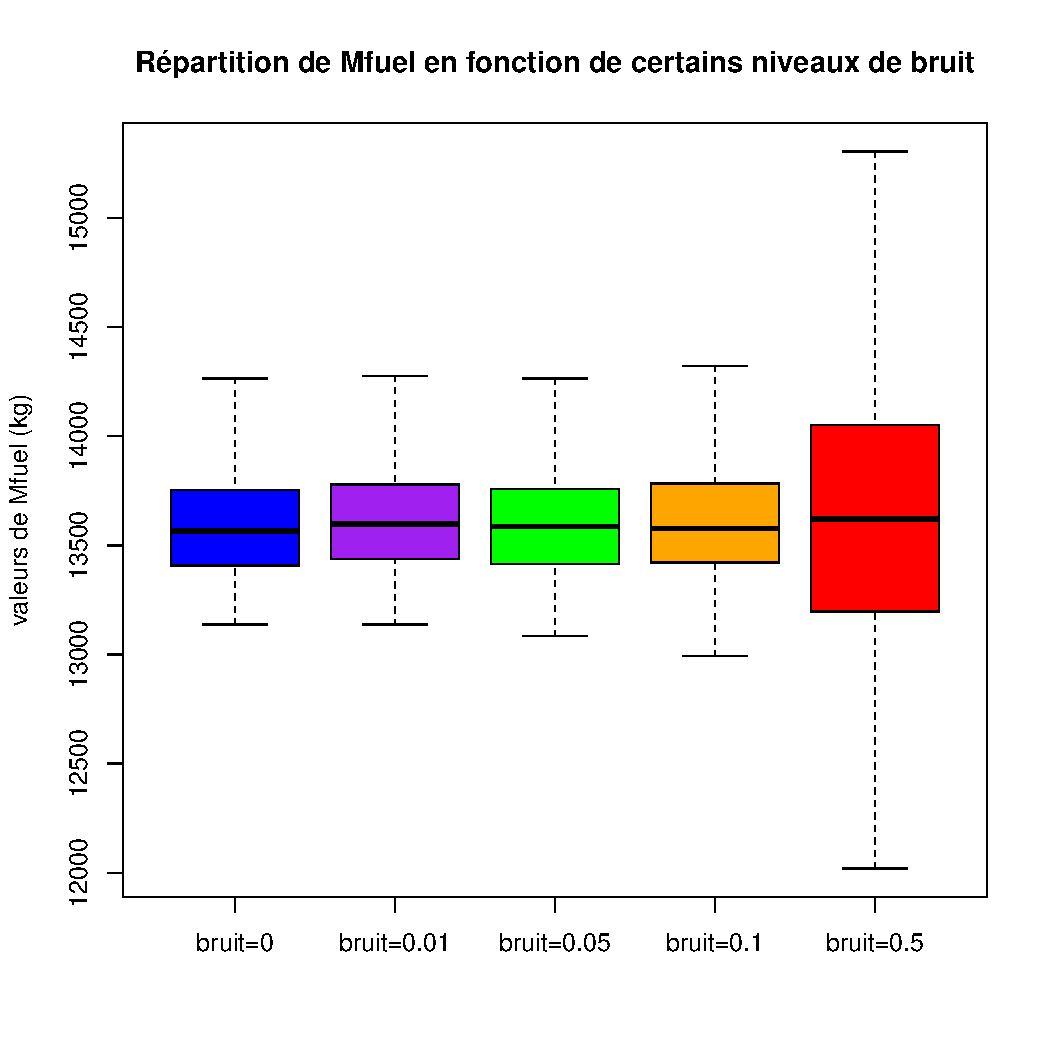
\includegraphics[scale=0.7]{boxplot.pdf}
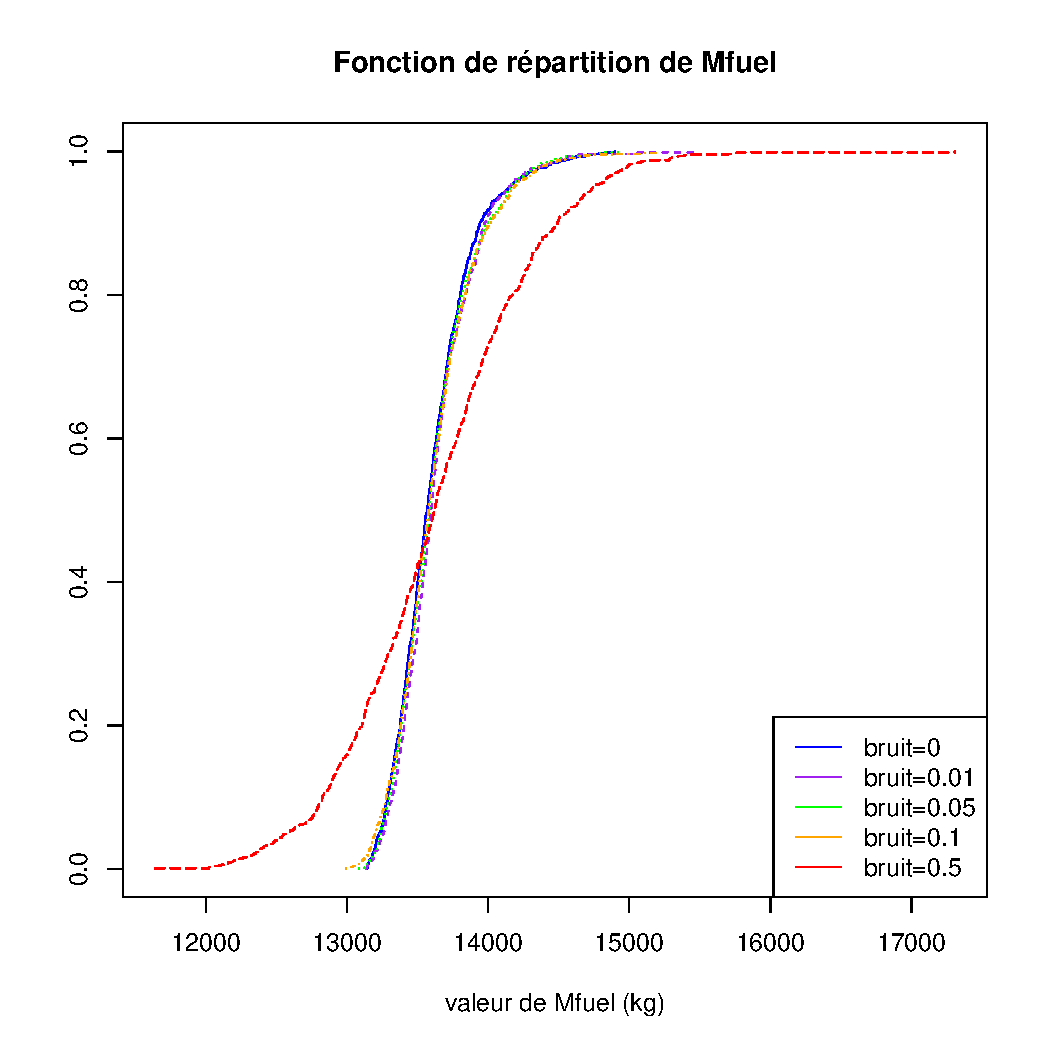
\includegraphics[scale=0.7]{M_fctrep_bruit.pdf}
\end{center}
La conclusion est la même que dans la partie 1 : $M_{fuel}$ semble peu sensible au bruit faible ($\sigma\approx 0.01$) mais très pour les bruits dépassant $\sigma=0.5$. La sensibilité de $M_{fuel}$ au bruitage des variables semble être exponentielle.
    
\chapter{Précision sur les indices de Sobol}  
Dans cette partie est décrite la matrice $\Gamma$ de la partie 2.2. Le document ~\cite{ref2} donne son expression termes à termes qui est ici adaptée à notre problème :


\begin{align*}
\begin{split}
\Gamma_{1,1} = \frac{1}{(\text{var}(M_{fuel}))^2}[\text{cov}(M_{fuel}M_{fuel}^{\{F\}},M_{fuel}M_{fuel}^{\{F\}}) - S^{\{F\}}\text{cov}(M_{fuel}M_{fuel}^{\{F\}},M_{fuel}^2) \\
- S^{\{F\}}\text{cov}(M_{fuel}M_{fuel}^{\{F\}},M_{fuel}^2) + S^{\{F\}}S^{\{F\}}\text{var}(M_{fuel})^2]
\end{split}
\end{align*}

\begin{align*}
\begin{split}
\Gamma_{1,2} = \frac{1}{(\text{var}(M_{fuel}))^2}[\text{cov}(M_{fuel}M_{fuel}^{\{F\}},M_{fuel}M_{fuel}^{\{SFC\}}) - S^{\{F\}}\text{cov}(M_{fuel}M_{fuel}^{\{SFC\}},M_{fuel}^2) \\
- S^{\{SFC\}}\text{cov}(M_{fuel}M_{fuel}^{\{F\}},M_{fuel}^2) + S^{\{SFC\}}S^{\{F\}}\text{var}(M_{fuel})^2]
\end{split}
\end{align*}

\begin{align*}
\begin{split}
\Gamma_{2,1} = \frac{1}{(\text{var}(M_{fuel}))^2}[\text{cov}(M_{fuel}M_{fuel}^{\{SFC\}},M_{fuel}M_{fuel}^{\{F\}}) - S^{\{SFC\}}\text{cov}(M_{fuel}M_{fuel}^{\{F\}},M_{fuel}^2)  \\
- S^{\{F\}}\text{cov}(M_{fuel}M_{fuel}^{\{SFC\}},M_{fuel}^2) + S^{\{F\}}S^{\{SFC\}}\text{var}(M_{fuel})^2]
\end{split}
\end{align*}

\begin{align*}
\begin{split}
\Gamma_{2,2} = \frac{1}{(\text{var}(M_{fuel}))^2}[\text{cov}(M_{fuel}M_{fuel}^{\{SFC\}},M_{fuel}M_{fuel}^{\{F\}}) - S^{\{F\}}\text{cov}(M_{fuel}M_{fuel}^{\{F\}},M_{fuel}^2) \\ 
- S^{\{SFC\}}\text{cov}(M_{fuel}M_{fuel}^{\{SFC\}},M_{fuel}^2) + S^{\{SFC\}}S^{\{SFC\}}\text{var}(M_{fuel})^2]
\end{split}
\end{align*}

  
\chapter{Précisions sur la régression linéaire multiple}

Voici quelques précisions sur le calcul de $R^2$. Il faut pour cela calculer quatre nombres :
\begin{enumerate}
\item[1.]La somme des carrés des résidus (SSE : sum of squared errors)
\[SSE=||\textbf{y-X\alpha}||^{2} (=5000.29)\]
\item[2.]La somme totale des carrés (SST : total sum of squares)
\[SST=||\textbf{y}-\bar{y}\textbf{1}||^{2}=\textbf{y}^{\textbf{T}}\textbf{y}-N\bar{y} (=39721761)\]
\item[3.]La somme des carrés de la régression (SSR : regression sum of squares) 
\[SSR=||\widehat{\textbf{y}}-\bar{y}\textbf{1}||^{2}=\alpha^{\textbf{T}}\textbf{X}^{\textbf{T}}\textbf{y}-N\bar{y} (=39713632)\]
Notons que $SST=SSR+SSE$
\item[4.]Le coefficient de détermination $R^{2}$
\[R^{2}=\frac{SSR}{SST} (=0.9997)\]
\end{enumerate}

\bigbreak
\bigbreak
\bigbreak
On propose aussi de préciser les estimations des coefficients de la régression linéaire multiple à l'aide du document ~\cite{ref3}. Celui-ci donne la méthode pour construire un intervalle de confiance autour de $a_i$ de niveau de sécurité $1-\alpha$. Cette démarche semble plus pertinente que l'énoncé d'uniques valeurs. On a :
\[IC_{1-\alpha}(a_i)=\textbf{a}_i\pm t_{1-\frac{\alpha}{2}}\sqrt{\hat{s^2}(\textbf{X}^{T}\textbf{X})^{-1}_{ii}}\]
où $t_{1-\frac{\alpha}{2}}$ est le $1-\frac{\alpha}{2}$-quantile de la distribution de $Student(N-p)$ ($N$ taille de l'échantillon, $p$ nombre de coefficients, ici $p=4$).

On trouve pour $\alpha=0.05$ :
\[a_0=28099.29\pm 98.56\]
\[a_1=-62.77\pm 0.10\]
\[a_2=-763.65\pm 5.00\]
\[a_3= 824.69\pm  0.78\]


\bibliography{bibli}
\bibliographystyle{plain}
\end{document}
